\documentclass[a4paper,1pt]{report}
\usepackage[utf8]{inputenc}
\usepackage[spanish]{babel}
\usepackage{amsfonts}
\usepackage{amsthm}
\usepackage{amssymb}
\usepackage{amsmath}
\usepackage{graphicx}
\usepackage{subcaption}
\usepackage{float}
\usepackage[rightcaption]{sidecap}
\usepackage[pdf]{graphviz}

\newtheorem*{pbo}{Principio del Buen Ordenamiento}

\newtheorem*{pim}{Principio de Inducción Matemática}

\newtheorem*{teo}{Teorema}

\newtheorem*{cor}{Corolario}

\newtheorem*{dem}{Demostración}

\newtheorem*{dfn}{Definición}

\newtheorem*{lem}{Lema}

\newtheorem*{prp}{Propiedades}


% Title Page
\title{Conferencia 9 - Maquinas de Turing}
\author{}

\begin{document}
\maketitle

\textbf{¿Cuáles son los problemas que pueden ser resueltos por algoritmos?}\\

Podemos definir como problema, de manera general, a calcular una función $f:\mathbb{N}^n\rightarrow \mathbb{N}$ 

\begin{dfn}[Función Calculable]
 Una función $f:\mathbb{N}^n\rightarrow \mathbb{N}$  es calculable~(computable) si:
 \begin{enumerate}
  \item Es total, o sea $Dom(f)=\mathbb{N}^n$
  \item Existe un procedimiento mecánico $P$ tal que dado $X=(x_1,x_2,\dots,x_n)$ se obtiene la respuesta
  de $f(X)$ en un número finito de pasos
 \end{enumerate}

\end{dfn}

\begin{dfn}[Función Parcialmente Calculable]
 Una función $f:\mathbb{N}^n\rightarrow \mathbb{N}$  es parcialmente calculable si:
 \begin{enumerate}
  \item Si $X\in Dom(f)$ entonces un procedimiento $P$ devuelve la respuesta $f(X)$ en un número finito 
  de pasos
  \item Si $X\not\in Dom(f)$ entonces el procedimiento $P$ no se detiene
 \end{enumerate}

\end{dfn}

\begin{dfn}[Alfabeto]
 Un alfabeto $\Sigma$ es un conjunto finito de símbolos
\end{dfn}

\begin{dfn}[Cadena]
 Una cadena~(palabra) es una secuencia finita de símbolos de un alfabeto
\end{dfn}

\begin{dfn}[Lenguaje]
 Un conjunto de cadenas sobre un alfabeto
\end{dfn}

Sobre un conjunto infinito de cadenas se puede hablar de:

\begin{itemize}
 \item Mecanismos generadores
 \item Mecanismos reconocedores
 \begin{itemize}
  \item Si: la cadena que recibe pertenece al lenguaje
  \item No: la cadena que recibe no pertenece al lenguaje
 \end{itemize}

\end{itemize}

\begin{dfn}
 Si $V$ es un lenguaje entonces $V^*$ son todas las cadenas que pueden obtenerse de $V$
\end{dfn}

Un tipo de procedimiento mecánico podría estar dado por: 
\begin{itemize}
 \item Una cinta unidimensional potencialmente infinita en ambas direcciones
 \item Un cabezal ubicado en una posición de la cinta , que puede desplazarse a la derecha o la izquierda, además de escribir en la cinta
 \item La cadena de entrada vendrá también en la cinta
 \item Una secuencia de instrucciones dadas en forma de estados con transiciones que indican a donde moverse y qué escribir en la cinta
\end{itemize}

A este procedimiento se le conoce como Máquina de Turing. A continuación se define formalmente.

\begin{dfn}[Maquina de Turing]
 Una Máquina de Turing es un séxtuplo $(Q,\gamma,\Sigma,\delta,q_0,F)$ donde:
 \begin{itemize}
  \item $Q$ : conjunto finito de estados
  \item $\gamma$: conjunto finito de símbolos de cinta~(alfabeto de cinta)
  \item $\Sigma$: alfabeto de entrada
  \item $\delta$: función de transición
  \item $q_0$: estado inicial
  \item $F$: estados finales
 \end{itemize}
\end{dfn}

\begin{dfn}
 $\delta$ se define como $\delta: Q\times\gamma \rightarrow Q\times\gamma\times\{I,D,P\}$ donde $I$ es moverse a la izquierda, $D$ moverse a la derecha y $P$ quedarse en la posición.
\end{dfn}

\textbf{Ejemplo:} $\delta(q_3,a)=(q_7,b,D)$ esto significa que se está parado en la cinta en el caracter a y en el etado $q_3$, escribo en la cinta el caracter b, cambio al estado $q_7$ y me muevo una casilla en la cinta a la derecha.

\begin{dfn}[Configuración]
 Una configuración es una terna $(q,c,i)$ donde\\ $q\in Q$, $c\in\gamma^*$ y $i\in\mathbb{N}$
\end{dfn}

\begin{dfn} 
Considere en una Máquina de Turing $T$ una transformación de la configuración $(q,c_1,i)$ en $(q',c_2,1)$ 
esto se denotaría como $(q,c_1,i)\vdash (q',c_2,1)$ ´
\end{dfn}

\textbf{Ejemplos:}
\\
 $\delta(q,S_i)=(q',S,D)\Rightarrow(q,S_1,S_2,\dots,S_n,i)\vdash(q',S_1,S_2,\dots,S_n,i+1)$\\
 $\delta(q,S_i)=(q',S,I)\Rightarrow(q,S_1,S_2,\dots,S_n,i)\vdash(q',S_1,S_2,\dots,S_n,i-1)$
 
 \begin{dfn}
  Una Máquina de Turing $T$ asume o reconoce una cadena $w$ si $(q,w,1)\overset{*}{\vdash}(q,S,i)$ donde
  $q\in F$, $S\in \gamma^*$ y $i \in \mathbb{N}$ y $\delta(q,S_i)$ no está definida.
 \end{dfn}

 $\overset{*}{\vdash}$ se define como: \textit{después de un conjunto finito de pasos se transforma en}\\
 
 Veamos varios ejemplos de Máquinas de Turing.\\
 
 Una Máquina de Turing~(1) que permite reconocer al lenguaje\\ 
 $L=\{w|w\in\{a,b\}^*$ tal que termina con $a\}$

 \begin{figure}[H]
        \centering
        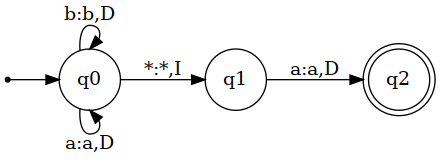
\includegraphics[width=0.6\textwidth]{figures9/tm1.png}
        \caption{Máquina de Turing 1}
\end{figure} 

\newpage
Noten como aquí se tienen los elementos del sextuplo:
\begin{itemize}
 \item $Q=\{q0,q1,q2\}$
 \item$q_0=q0$
 \item $F=\{q2\}$
 \item $\gamma=\{a,b,*\}$
 \item $\Sigma=\{a,b\}$
 \item $\delta(q0,b)=(b,D,q0)$, $\delta(q0,a)=(a,D,q0)$, $\delta(q0,*)=(*,I,q1)$,\\ $\delta(q1,a)=(a,P,q2)$ 
\end{itemize}


Una Máquina de Turing~(2) que permite reconocer al lenguaje\\ 
 $L=\{0^n,1^n|n\geq 1\}$

 \begin{figure}[H]
        \centering
        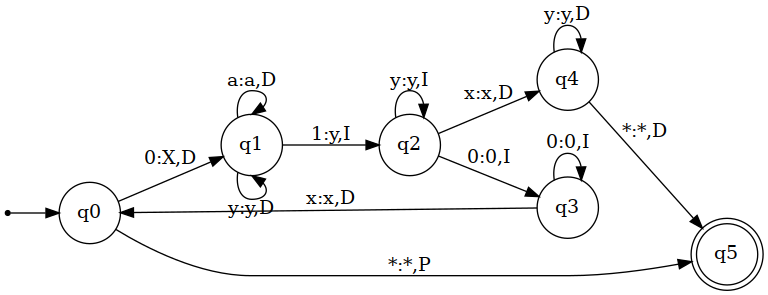
\includegraphics[width=1.1\textwidth]{figures9/tm2.png}
        \caption{Máquina de Turing 2}
\end{figure} 


Las Máquinas de Turing también se utilizan no solo para reconcer lenguajes, sino también para computar funciones. En estos casos la salida es lo que se deja escrito en la cinta.\\

Un ejemplo es computar $f(x)=x+1$. Una idea aquí es representar la entrada como 1's consecutivos.

 \begin{figure}[H]
        \centering
        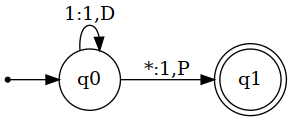
\includegraphics[width=0.4\textwidth]{figures9/tm3.png}
        \caption{Máquina de Turing 3}
\end{figure} 

\newpage

Otro ejemplo es computar $f(x,y)=x+y$. Aquí de nuevo cada número se representar en la entrada como 1's consecutivos pero se toma al 0 como separador entre números.


 \begin{figure}[H]
        \centering
        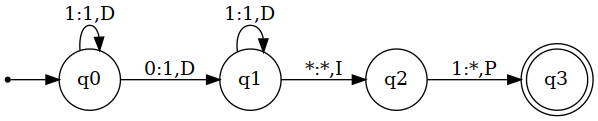
\includegraphics[width=0.8\textwidth]{figures9/tm4.png}
        \caption{Máquina de Turing 4}
\end{figure} 
  
\end{document} 
